%\documentclass[a4paper]{article}
%% Language and font encodings
\documentclass[twocolumn,aps,prl]{revtex4-1}
\usepackage[utf8]{inputenc}
\usepackage[spanish, es-tabla]{babel}
\usepackage[T1]{fontenc}
\usepackage{amsmath}
\usepackage{amssymb}
\usepackage{siunitx}
\usepackage{multirow}
\usepackage{float}
\usepackage{enumitem} % enumerar

\sisetup{math-micro=\text{µ},text-micro=µ}

\usepackage[toc,page]{appendix}

%% Sets page size and margins
\usepackage[a4paper,top=1.5cm,bottom=2cm,left=1.7cm,right=1.7cm,marginparwidth=1.75cm]{geometry}

%% Sets caption text size(its bigger than text)
\usepackage{caption}
\captionsetup[figure]{font=small}
\usepackage{subcaption}

%% Useful packages
\usepackage{svg}
\usepackage{epstopdf}
\usepackage{amsmath}
\usepackage{graphicx}
\usepackage[colorlinks=true, allcolors=blue]{hyperref}

\newcommand{\nstar}{n^*} 
\newcommand{\Nstar}{N^*} 

\newcommand*\sepline{%
  \begin{center}
    \rule[1ex]{.5\textwidth}{.5pt}
  \end{center}}

%%%%%%%%%%%%%%%%%%%%%%%%%%%%%%%%%%%%%%%%%%%%%%%%%%%%%%
%%%%%%%%%%%%%%%%%%%%%%%%%%%%%%%%%%%%%%%%%%%%%%%%%%%%%%
%%%%%%%%%%%%%%%%%%%%%%%%%%%%%%%%%%%%%%%%%%%%%%%%%%%%%%
%%%%%%%%%%%%%%%%%%%%%%%%%%%%%%%%%%%%%%%%%%%%%%%%%%%%%%
%%%%%%%%%%%%%%%%%%%%%%%%%%%%%%%%%%%%%%%%%%%%%%%%%%%%%%

\begin{document}

% ██   ██ ███████  █████  ██████
% ██   ██ ██      ██   ██ ██   ██
% ███████ █████   ███████ ██   ██
% ██   ██ ██      ██   ██ ██   ██
% ██   ██ ███████ ██   ██ ██████

\title{Práctico 2}
\author{M. G. Aramayo}
\affiliation{Matemática de sistemas biológicos, Instituto Balseiro}

% \begin{abstract}
% Mete acá las conclusiones.
% \end{abstract}

\maketitle


% ███████╗██╗  ██╗ ██╗
% ██╔════╝╚██╗██╔╝███║
% █████╗   ╚███╔╝ ╚██║
% ██╔══╝   ██╔██╗  ██║
% ███████╗██╔╝ ██╗ ██║
% ╚══════╝╚═╝  ╚═╝ ╚═╝

\section{Resolución Ej 1:}

% \begin{figure}
%     \centering
%     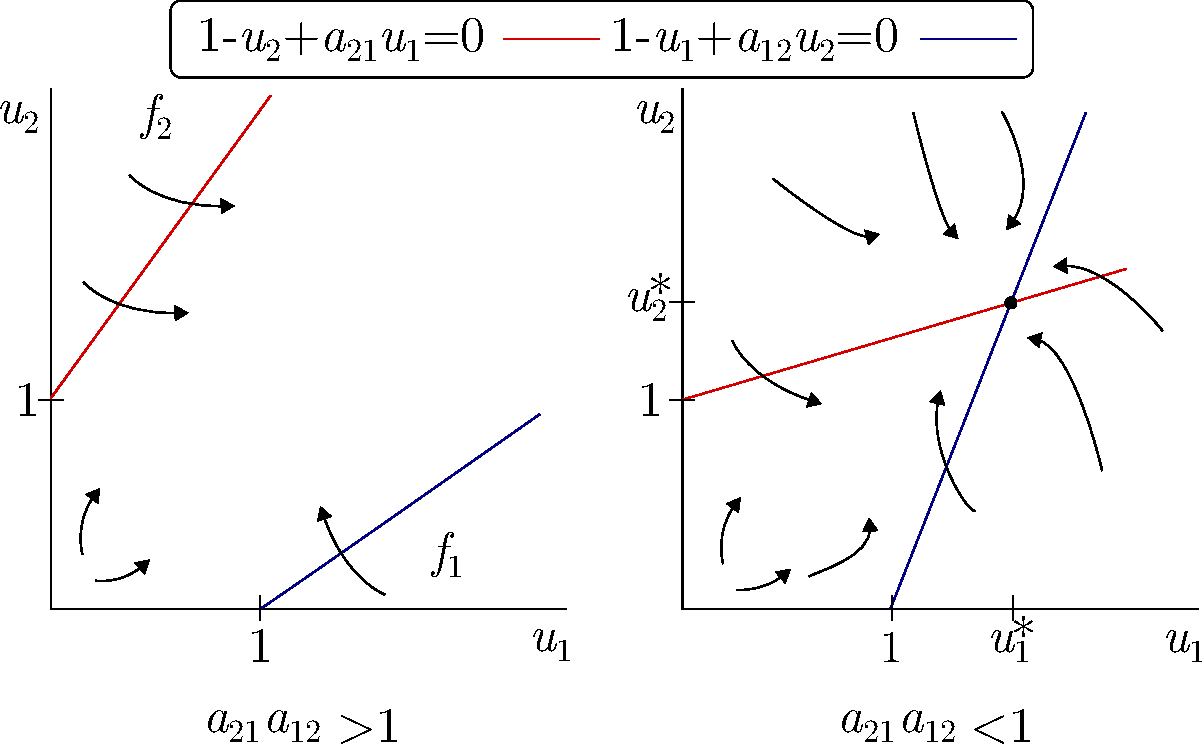
\includegraphics[width=0.5\textwidth]{figuras/equilibrio.pdf}
%     \caption{a.}
%     \label{fig:mosquitos}
% \end{figure}


% ███████╗ ██████╗ ██╗
% ██╔════╝██╔════╝███║
% █████╗  ██║     ╚██║
% ██╔══╝  ██║      ██║
% ███████╗╚██████╗ ██║
% ╚══════╝ ╚═════╝ ╚═╝

Analizando la dinámica del sistema:

$$ \left\lbrace
\begin{aligned}
  \dot{x} &= f_1(x,y,z) = x \left[(A \vec{x})_{x}-\vec{x} \cdot A \vec{x}\right] \\
  \dot{y} &= f_2(x,y,z) = y \left[(A \vec{x})_{y}-\vec{x} \cdot A \vec{x}\right] \\
  \dot{z} &= f_3(x,y,z) = z \left[(A \vec{x})_{z}-\vec{x} \cdot A \vec{x}\right]
\end{aligned}
\right.
$$

Reduciendo a dos variables mediante la condición. $z = 1-x-y$

\sepline

Para el primer sistema y su correspondiente matriz de payoff

$$
Ax = 
\begin{pmatrix}
    \frac{g-c}{2}&g&\frac{g-c}{2}\\
    0&\frac{g}{2}&\frac{g}{2}\\
    \frac{g-c}{2}&\frac{g}{2}&\frac{g}{2}
\end{pmatrix}
\begin{pmatrix}
    x\\
    y\\ 
    1-x-y
\end{pmatrix}
=
\begin{pmatrix}
    \frac{gy+g-c+cy}{2}\\ 
    \frac{g-gx}{2}\\ 
    \frac{g-cx}{2}
\end{pmatrix}
$$

$$(Ax)_x = \frac{gy+g-c+cy}{2}
,\quad 
(Ax)_y = \frac{g-gx}{2}
$$

$$
x^T Ax = \frac{cx^2-2cx+2cxy+g}{2}
$$

$$
f_1(x, y) = 
-x \frac{
    cx^2
    + 2cyx
    - 2cx
    - gy
    - cy
    + c
    }{2}
$$

$$
f_2(x, y) = 
-xy \frac{cx+2cy+g-2c}{2}
$$

% $$
% c((2-(g/c))-2y)^2
% + 2cy((2-(g/c))-2y)
% - 2c((2-(g/c))-2y)
% - gy
% - cy
% + c
% $$

% $$ \left\lbrace
% \begin{aligned}
%   \dot{x} &= x \left[(A \vec{x})_{x}-\vec{x} \cdot A \vec{x}\right] \\
%   \dot{y} &= y \left[(A \vec{x})_{y}-\vec{x} \cdot A \vec{x}\right] \\
%   \dot{z} &= z \left[(A \vec{x})_{z}-\vec{x} \cdot A \vec{x}\right]
% \end{aligned}
% \right.
% $$

Puntos de equilibrio:

\begin{itemize}
    \item[] $P_1^* = (0, \frac{G-2C}{2C}, 1 - \frac{G-2C}{2C})$
    \item[] $P_2^* = (0, 0, 1)$
    \item[] $P_3^* = (0, \frac{C}{G+C}, 1 - \frac{C}{G+C})$
    \item[] $P_4^* = (1, 0, 0)$
    \item[] $P_5^* = (\frac{G}{C}, 1- \frac{G}{C}, 0)$
\end{itemize}

% $$ J =
% \begin{pmatrix}
%     \frac{\partial }{\partial x}\left(-x\frac{cx^2+2cyx-2cx-gy-cy+c}{2}\right) 
%     &
%     \frac{\partial }{\partial y}\left(-x\frac{cx^2+2cyx-2cx-gy-cy+c}{2}\right)
%     \\  
%     \frac{\partial }{\partial x}\left(-xy\frac{cx+2cy+g-2c}{2}\right)          
%     &
%     \frac{\partial }{\partial y}\left(-xy\frac{cx+2cy+g-2c}{2}\right)
% \end{pmatrix}
% $$

% $$J =
% \begin{pmatrix}
%     -\frac{3cx^2-4cx+4cxy+c-gy-cy}{2}
%     &
%     -\frac{x\left(2cx-c-g\right)}{2}
%     \\  
%     -\frac{y\left(2cx-2c+g+2cy\right)}{2}
%     &
%     -\frac{x\left(4cy-2c+g+cx\right)}{2}
% \end{pmatrix}
% $$

% $$J_1 =
% \begin{pmatrix}
%     -\frac{3c(0)^2-4c(0)+4c(0)(\frac{g-2c}{2c})+c-g(\frac{g-2c}{2c})-c(\frac{g-2c}{2c})}{2}
%     &
%     -\frac{(0)\left(2c(0)-c-g\right)}{2}
%     \\  
%     -\frac{(\frac{g-2c}{2c})\left(2c(0)-2c+g+2c(\frac{g-2c}{2c})\right)}{2}
%     &
%     -\frac{(0)\left(4c(\frac{g-2c}{2c})-2c+g+c(0)\right)}{2}
% \end{pmatrix}
% $$

% $$J_1 =
% \begin{pmatrix}
%     -\frac{-g^2+cg+4c^2}{4c}
%     &
%     0
%     \\  
%     -\frac{\left(g-2c\right)^2}{2c}
%     &
%     0
% \end{pmatrix}
% $$


$$J_1 =
\begin{pmatrix}
    -\frac{-g^2+cg+4c^2}{4c}
    &
    0
    \\  
    -\frac{\left(g-2c\right)^2}{2c}
    &
    0
\end{pmatrix}
\Rightarrow \text{Acumulación}
$$


% $$J_2 =
% \begin{pmatrix}
%     -\frac{3c(0)^2-4c(0)+4c(0)(0)+c-g(0)-c(0)}{2}
%     &
%     -\frac{(0)\left(2c(0)-c-g\right)}{2}
%     \\  
%     -\frac{(0)\left(2c(0)-2c+g+2c(0)\right)}{2}
%     &
%     -\frac{(0)\left(4c(0)-2c+g+c(0)\right)}{2}
% \end{pmatrix}
% $$

% $$J_2=
% \begin{pmatrix}
%     -\frac{3c(0)^2-4c(0)+4c(0)(0)+c-g(0)-c(0)}{2}
%     &
%     -\frac{(0)\left(2c(0)-c-g\right)}{2}
%     \\  
%     -\frac{(0)\left(2c(0)-2c+g+2c(0)\right)}{2}
%     &
%     -\frac{(0)\left(4c(0)-2c+g+c(0)\right)}{2}
% \end{pmatrix}
% $$

$$J_2=
\begin{pmatrix}
    -\frac{c}{2}
    &
    0
    \\  
    0
    &
    0
\end{pmatrix}
\Rightarrow \text{Acumulación de estables} 
$$

% $$J_3 =
% \begin{pmatrix}
%     -\frac{3c(0)^2-4c(0)+4c(0)(\frac{c}{g+c})+c-g(\frac{c}{g+c})-c(\frac{c}{g+c})}{2}
%     &
%     -\frac{(0)\left(2c(0)-c-g\right)}{2}
%     \\  
%     -\frac{(\frac{c}{g+c})\left(2c(0)-2c+g+2c(\frac{c}{g+c})\right)}{2}
%     &
%     -\frac{(0)\left(4c(\frac{c}{g+c})-2c+g+c(0)\right)}{2}
% \end{pmatrix}
% $$

$$J_3 =
\begin{pmatrix}
    0
    &
    0
    \\  
    -\frac{c\left(g^2-cg\right)}{2\left(g+c\right)^2}
    &
    0
\end{pmatrix}
\Rightarrow Saddle ??????
$$



% $$J_4 =
% \begin{pmatrix}
%     -\frac{3c(1)^2-4c(1)+4c(1)(0)+c-g(0)-c(0)}{2}
%     &
%     -\frac{(1)\left(2c(1)-c-g\right)}{2}
%     \\  
%     -\frac{(0)\left(2c(1)-2c+g+2c(0)\right)}{2}
%     &
%     -\frac{(1)\left(4c(0)-2c+g+c(1)\right)}{2}
% \end{pmatrix}
% $$

$$J_4 =
\begin{pmatrix}
    0
    &
    -\frac{-g+c}{2}
    \\  
    0
    &
    -\frac{g-c}{2}
\end{pmatrix}
\Rightarrow \text{Acumulación de } ^{\text{Estables si } g>c}_{\text{Inestables si } g<c}
$$

% $$J_5 =
% \begin{pmatrix}
%     -\frac{3c(\frac{g}{c})^2-4c(\frac{g}{c})+4c(\frac{g}{c})(1 - \frac{g}{c})+c-g(1 - \frac{g}{c})-c(1 - \frac{g}{c})}{2}
%     &
%     -\frac{(\frac{g}{c})\left(2c(\frac{g}{c})-c-g\right)}{2}
%     \\  
%     -\frac{(1 - \frac{g}{c})\left(2c(\frac{g}{c})-2c+g+2c(1 - \frac{g}{c})\right)}{2}
%     &
%     -\frac{(\frac{g}{c})\left(4c(1 - \frac{g}{c})-2c+g+c(\frac{g}{c})\right)}{2}
% \end{pmatrix}
% $$

$$J_5 =
\begin{pmatrix}
    0
    &
    -\frac{g\left(g-c\right)}{2c}
    \\  
    -\frac{g\left(-g+c\right)}{2c}
    &
    -\frac{g\left(-g+c\right)}{c}
\end{pmatrix}
\Rightarrow  \lambda_{1,2} = \frac{g}{c} \frac{g-c}{2}
% \Rightarrow \text{Equilibrio }  ^{\text{Estables si } g<c}_{\text{Inestables si } g>c}
$$

$$
\Rightarrow \text{Equilibrio }  ^{\text{Estables si } g<c}_{\text{Inestables si } g>c}
$$


% ███████╗ ██████╗    ██████╗ 
% ██╔════╝██╔════╝    ╚════██╗
% █████╗  ██║          █████╔╝
% ██╔══╝  ██║         ██╔═══╝ 
% ███████╗╚██████╗    ███████╗
% ╚══════╝ ╚═════╝    ╚══════╝

\sepline

Para el segundo sistema

$$
Ax =
\begin{pmatrix}
    \frac{g-c}{2}&g&g\\ 
    0&\frac{g}{2}&0\\ 
    0&g&\frac{g}{2}
\end{pmatrix}
\begin{pmatrix}
    x\\
    y\\ 
    1-x-y
\end{pmatrix}
=
\begin{pmatrix}
    \frac{-gx+2g-cx}{2}\\ 
    \frac{gy}{2}\\ 
    \frac{-gx+gy+g}{2}
\end{pmatrix}
$$


$$
(Ax)_x = \frac{-gx+2g-cx}{2}
, \quad 
(Ax)_y = \frac{gy}{2}
, \quad 
x^T Ax = \frac{g-cx^2}{2}
$$

$$
f_1(x, y) 
% = 
% x
% \frac{-xg+g+cx^2-cx}{2} 
= 
\frac{x}{2} (
    cx^2
    -x(g+c)
    +g
    )
$$

$$
f_2(x, y) 
% = y
% \frac{gy-g+cx^2}{2} 
=
\frac{y}{2} (cx^2+gy-g)
$$

% $$ \left\lbrace
% \begin{aligned}
%   \dot{x} &= x \left[(A \vec{x})_{x}-\vec{x} \cdot A \vec{x}\right] \\
%   \dot{y} &= y \left[(A \vec{x})_{y}-\vec{x} \cdot A \vec{x}\right] \\
%   \dot{z} &= z \left[(A \vec{x})_{z}-\vec{x} \cdot A \vec{x}\right]
% \end{aligned}
% \right.
% $$

Puntos de equilibrio:

\begin{itemize}
    \item[] $P_1^* = (0, 0, 1 )$
    \item[] $P_2^* = (0, 1, 0)$
    \item[] $P_3^* = (1, 0, 0)$
    \item[] $P_4^* = (\frac{G}{C}, 0, 1- \frac{G}{C})$
\end{itemize}

% $$ J =
% \begin{pmatrix}
%     \frac{\partial }{\partial x}\left(\frac{x}{2} (cx^2-x(g+c)+g)\right)
%     &
%     \frac{\partial }{\partial y}\left(\frac{x}{2} (cx^2-x(g+c)+g)\right)
%     \\  
%     \frac{\partial }{\partial x}\left(\frac{y}{2} (cx^2+gy-g)\right)          
%     &
%     \frac{\partial }{\partial y}\left(\frac{y}{2} (cx^2+gy-g)\right)
% \end{pmatrix}
% $$

% $$ J =
% \begin{pmatrix}
%     \frac{3x^2c-2xc-2xg+g}{2}
%     &
%     0
%     \\  
%     cyx
%     &
%     \frac{2gy-g+cx^2}{2}
% \end{pmatrix}
% $$

$$ J_1 =
\begin{pmatrix}
    \frac{g}{2}
    &
    0
    \\  
    0
    &
    -\frac{g}{2}
\end{pmatrix}
\Rightarrow Saddle
$$

$$ J_2 =
\begin{pmatrix}
    \frac{g}{2}
    &
    0
    \\  
    0
    &
    \frac{g}{2}
\end{pmatrix}
\Rightarrow \text{Inestable}
$$

$$ J_3 =
\begin{pmatrix}
    \frac{c-g}{2}
    &
    0
    \\  
    0
    &
    \frac{c-g}{2}
\end{pmatrix}
\Rightarrow \text{Equilibrio }  ^{\text{Estables si } g>c}_{\text{Inestables si } g<c}
$$

$$ J_4 =
\begin{pmatrix}
    \frac{g}{c} \frac{g-c}{2}
    &
    0
    \\  
    0
    &
    \frac{g}{c} \frac{g-c}{2}
\end{pmatrix}
\Rightarrow \text{Equilibrio }  ^{\text{Estables si } g<c}_{\text{Inestables si } g>c}
$$

% ███████╗██╗  ██╗    ██████╗  
% ██╔════╝╚██╗██╔╝    ╚════██╗
% █████╗   ╚███╔╝      █████╔╝
% ██╔══╝   ██╔██╗     ██╔═══╝ 
% ███████╗██╔╝ ██╗    ███████╗
% ╚══════╝╚═╝  ╚═╝    ╚══════╝

\section{Resolución Ej 2:}


%%%%%%%%%%%%%%%%%%%%%%%%%%%%%%%%%%%%%%%%%%%%%%%%%%%%%%%%%%%%%%%%%%%%%%
\sepline
%%%%%%%%%%%%%%%%%%%%%%%%%%%%%%%%%%%%%%%%%%%%%%%%%%%%%%%%%%%%%%%%%%%%%%


% ███████╗██╗  ██╗    ██████╗     
% ██╔════╝╚██╗██╔╝    ╚════██╗    
% █████╗   ╚███╔╝      █████╔╝    
% ██╔══╝   ██╔██╗      ╚═══██╗    
% ███████╗██╔╝ ██╗    ██████╔╝    
% ╚══════╝╚═╝  ╚═╝    ╚═════╝     

\section{Resolución Ej 3:}

% \bibliography{sample}

\end{document}

% ███    ██  ██████  ████████  █████  ███████
% ████   ██ ██    ██    ██    ██   ██ ██
% ██ ██  ██ ██    ██    ██    ███████ ███████
% ██  ██ ██ ██    ██    ██    ██   ██      ██
% ██   ████  ██████     ██    ██   ██ ███████


% ████████ ██    ██ ██████   ██████  ███████
%    ██     ██  ██  ██   ██ ██    ██ ██
%    ██      ████   ██████  ██    ██ ███████
%    ██       ██    ██      ██    ██      ██
%    ██       ██    ██       ██████  ███████

% atomico
% volumen
% parametro
% mantenia
% dielectrico
% perdida
% ferroelectrico
% difractograma
% difractometro
% minimo
% maximo
% tension
% conversion
% aislacion
% medicion
% resolucion
% funcion
% transicion
% correccion
% activacion
% correlacion
% tipico X
% habia  X
% agrego X
